\documentclass[10pt]{beamer}
\usepackage[utf8]{inputenc}
\usepackage{graphicx}
\usepackage {mathtools}
\usepackage{hyperref}
\usepackage{hyperref}
\usepackage{utopia} %font utopia imported
\usetheme{CambridgeUS}
\usecolortheme{dolphin}
\hypersetup{colorlinks=true,linkcolor=blue, linktocpage}
% set colors
\definecolor{myNewColorA}{RGB}{118,193,188}
\definecolor{myNewColorB}{RGB}{106,172,150}
\definecolor{myNewColorC}{RGB}{94,150,218}
\setbeamercolor*{palette primary}{bg=myNewColorC}
\setbeamercolor*{palette secondary}{bg=myNewColorB, fg=white}
\setbeamercolor*{palette tertiary}{bg=myNewColorA, fg=white}
\setbeamercolor*{titlelike}{fg=myNewColorA}
\setbeamercolor*{title}{bg=myNewColorA, fg=white}
\setbeamercolor*{item}{fg=myNewColorA}
\setbeamercolor*{caption name}{fg=myNewColorA}
\usefonttheme{professionalfonts}
\usepackage{natbib}
\usepackage{hyperref}
%------------------------------------------------------------
\titlegraphic{\includegraphics[height=1.5cm]{../../CommonFigures/Universidad_Panamericana-logo.jpg}}

\setbeamerfont{title}{size=\large}
\setbeamerfont{subtitle}{size=\small}
\setbeamerfont{author}{size=\small}
\setbeamerfont{date}{size=\small}
\setbeamerfont{institute}{size=\small}
\title[Universidad Panamericana]{}
\subtitle{Introduction to Real-Time Operating Systems}
\author[]{Name}

\institute[ltonix@up.edu.mx]{Universidad Panamericana}
\date[Presentation \today]
{Presentation \today}

%------------------------------------------------------------
%This block of commands puts the table of contents at the 
%beginning of each section and highlights the current section:
%\AtBeginSection[]
%{
%  \begin{frame}
%    \frametitle{Contents}
%    \tableofcontents[currentsection]
%  \end{frame}
%}
\AtBeginSection[]{
  \begin{frame}
  \vfill
  \centering
  \begin{beamercolorbox}[sep=8pt,center,shadow=true,rounded=true]{title}
    \usebeamerfont{title}\insertsectionhead\par%
  \end{beamercolorbox}
  \vfill
  \end{frame}
}
\setbeamercolor{block title}{bg=myNewColorA, fg=black} % Background and foreground colors for the block title
\setbeamercolor{block body}{bg=myNewColorC, fg=black} % Background and foreground colors for the block body
%------------------------------------------------------------

\begin{document}

%The next statement creates the title page.
\frame{\titlepage}
\begin{frame}
\frametitle{Contents}
\tableofcontents
\end{frame}
%------------------------------------------------------------
\section{What is an operating system?}
    \begin{frame}{What is an operating system?}
      
      \begin{block}{Block Title}
        \textbf{Is a software that manages and distributes multiple running applications} across a computer or platform, with the main objective to \textbf{efficiently manage multiple tasks simultaneously}.
      \end{block}
      \begin{itemize}
        \item It acts as a mediator between the computer's hardware and the applications that run on it, providing a user-friendly interface and managing the execution of software programs.
      \end{itemize}
    \end{frame}
\subsection{Main features of an OS}
%------------------------------------------------------------   
    \begin{frame}{Modularity}
      \begin{itemize}
        \item Modularity: Operating systems should be modular in design, allowing for parts of the system to be modified or enhanced without affecting other parts. This supports easier updates and maintenance.
        \begin{figure}[h]
          \centering
          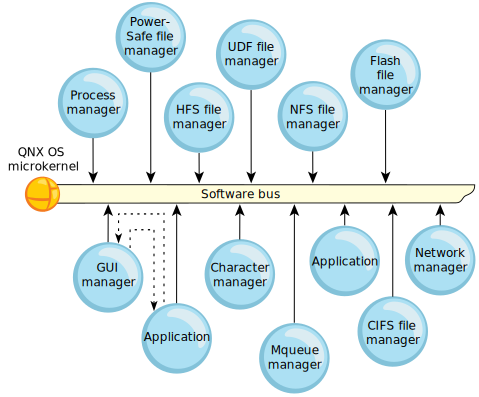
\includegraphics[width=0.5\textwidth]{figures/qnxOSExample.png}
          \caption{Here is the caption of the figure.}
          \label{fig:my_label}
          \end{figure}
      \end{itemize}
    \end{frame}
%------------------------------------------------------------ 
    \begin{frame}{Portability, Usability, and Responsiveness}
      \begin{itemize}
      \item \textbf{Portability}: The ability of the operating system to run on different types of hardware without significant modifications. This is crucial for reducing the development time and cost when moving software among different systems.
      \item \textbf{Usability}: The operating system should be designed for ease of use, with interfaces and tools that are intuitive and easy to learn for various categories of users.
      \item \textbf{Responsiveness}: The system should respond in a timely manner to user inputs and system events. This is particularly important in interactive environments and real-time operating systems.
      \item $\rightarrow$ \href{https://www.youtube.com/watch?v=R_FoFbAyVQk\#t=10s}{Check the video}
    \end{itemize}
    \end{frame}
    \subsection{Safety}
    \begin{frame}{Safety in Operating Systems}
      \begin{block}{Definition of Safety}
          Ensuring that an operating system operates without leading to catastrophic consequences in the environment it controls.
      \end{block}
      \begin{block}{Objectives}
          \begin{itemize}
              \item Prevent system failures that might lead to hazardous situations.
              \item Ensure reliability and fault tolerance.
          \end{itemize}
      \end{block}
      \begin{block}{Strategies}
          \begin{itemize}
              \item Redundancy in critical system components.
              \item Regular system audits and error checks.
              \item Use of watchdog timers to recover from hardware/software failures.
          \end{itemize}
      \end{block}
  \end{frame}
  \subsection{Security}
  \begin{frame}{Security in Operating Systems}
    \begin{block}{Definition of Security}
        Protecting system resources and data from unauthorized access and ensuring confidentiality, integrity, and availability.
    \end{block}
    \begin{block}{Objectives}
        \begin{itemize}
            \item Protect data confidentiality and integrity.
            \item Ensure system availability against attacks and breaches.
        \end{itemize}
    \end{block}
    \begin{block}{Strategies}
        \begin{itemize}
            \item Implementation of user authentication mechanisms.
            \item Use of encryption for data protection.
            \item Regular updates and patches to fix vulnerabilities.
        \end{itemize}
    \end{block}
\end{frame}



\subsection{What is real time?}
\begin{frame}{What is a Real-Time Operating System (RTOS)?}
  \begin{itemize}
      \item \textbf{Purpose:} Real-time systems are designed to respond to input or events within a guaranteed time frame, typically measured in milliseconds or microseconds. The term "real-time" refers to the system’s ability to process and respond to inputs almost instantaneously, ensuring outputs are produced within a strictly defined time period relative to an event.
      \item \textbf{Deterministic:} Behavior in terms of timing and execution is predictable.
      \item \textbf{Use Cases:}
          \begin{itemize}
              \item Embedded systems (e.g., medical devices, automotive controls)
              \item Industrial automation
              \item Telecommunications systems
          \end{itemize}
  \end{itemize}
\end{frame}

\begin{frame}{What is a Real-Time Operating System (RTOS)?}
  \begin{figure}[h]
    \centering
    \includegraphics[width=1.0\textwidth]{figures/real_time_tasks.png}
    \label{fig:my_label}
    \end{figure}
\end{frame}

\section{Open Source}
    \begin{frame}{Terms of service you didn't read }
      \begin{itemize}
        \item Blizard
        \item Paypal
        \item Pinterest
        \item Facebook
      \end{itemize}
      \begin{alertblock}{Important}
        Thats why open source is soo important \newline
        \href{https://tosdr.org/}{Click}
      \end{alertblock}
      \begin{figure}[h]
        \centering
        \includegraphics[width=0.5\textwidth]{figures/DoxingMeme.jpg}
        \label{fig:my_label}
        \end{figure}
    \end{frame}

    \begin{frame}{Introduction to Open Source Licenses}
      \begin{itemize}
          \item Open source licenses empower developers to access, modify, and share software code.
          \item They promote collaboration and innovation in the software development community.
          \item Different licenses come with different permissions, conditions, and limitations.
      \end{itemize}
  \end{frame}
  \subsection{MIT License}
  \begin{frame}{The MIT License}
    \begin{itemize}
        \item \textbf{Overview:} One of the most permissive open source licenses.
        \item \textbf{Permissions:} 
            \begin{itemize}
                \item Allows commercial use, modification, distribution, private use.
                \item Minimal restrictions on how software can be redistributed.
            \end{itemize}
        \item \textbf{Requirements:}
            \begin{itemize}
                \item License and copyright notice must be included with copies of the software.
            \end{itemize}
        \item \textbf{Key Feature:} Does not require derivative works to be distributed under the same license.
    \end{itemize}
\end{frame}
\subsection{GNU}
\begin{frame}{The GNU General Public License (GPL)}
    \begin{itemize}
        \item \textbf{Overview:} A copyleft license that requires derivatives to be open.
        \item \textbf{Permissions:}
            \begin{itemize}
                \item Permits commercial use, modification, distribution, and private use.
            \end{itemize}
        \item \textbf{Requirements:}
            \begin{itemize}
                \item Derived works must be released under the same license (GPL).
                \item Must accompany with the source code or offer access to the source.
            \end{itemize}
        \item \textbf{Key Feature:} Ensures that the freedom to modify and redistribute is preserved in derivatives, known as "share-alike".
    \end{itemize}
\end{frame}
\subsection{Comparison of MIT and GPL}
\begin{frame}{Comparison of MIT and GPL}
    \begin{itemize}
        \item \textbf{MIT License:} Encourages widespread use and modification without requiring derivatives to use the same license.
        \item \textbf{GPL:} Promotes free use but enforces that any derivative work must also be freely available under the GPL, preserving the original freedoms.
    \end{itemize}
\end{frame}
\subsection{Understanding Copyleft}

\begin{frame}{Understanding Copyleft}
\textcolor{myNewColorA}{\Huge{\centerline{\href{https://www.fsf.org/blogs/community/help-others-find-free-software-watch-and-share-escape-to-freedom}{FreeSoftwareVideo}}}}

\end{frame}

\begin{frame}{Understanding Copyleft}
  \begin{itemize}
      \item \textbf{Definition:} Copyleft is a licensing scheme that allows the software (and sometimes other types of works) to be freely used, modified, and distributed, but with one key condition: any derivative work must also be distributed under the same or compatible copyleft terms.
      
      \item \textbf{Purpose:} The main goal of copyleft is to ensure that all versions of the software remain free and open, preventing proprietary forks that restrict user freedoms.
      
      \item \textbf{Key Features:}
          \begin{itemize}
              \item \textit{Viral Nature:} The copyleft clause is often described as "viral" because it requires all modified and extended versions of the program to be free as well.
              \item \textit{Share and Share Alike:} If you distribute copies or modified versions, you must also share the source code under the same terms.
          \end{itemize}
      
      \item \textbf{Examples of Copyleft Licenses:}
          \begin{itemize}
              \item GNU General Public License (GPL)
              \item GNU Lesser General Public License (LGPL)
              \item Mozilla Public License (MPL)
          \end{itemize}
  \end{itemize}
\end{frame}

\subsection{Comparison of Open Source Licenses}
\begin{frame}{Comparison of Open Source Licenses}
  \footnotesize % You can use \tiny, \scriptsize, or \footnotesize as well
  \begin{table}[]
      \begin{tabular}{|l|l|l|}
      \hline
      \textbf{License} & \textbf{Characteristics} & \textbf{Ownership Potential} \\ \hline
      MIT              & Very permissive, minimal requirements & \alert{High(Proprietary possible)}  \\ \hline
      BSD              & Similar to MIT, slightly more clauses & \alert{High(Proprietary possible)}  \\ \hline
      GPL              & Copyleft,requires same license on derivatives & Low (Must remain open) \\ \hline
      Apache           & Permissive, includes patent clauses & Moderate (Proprietary with conditions) \\ \hline
      \end{tabular}
  \end{table}

  \begin{alertblock}{Note}
      Licenses marked with \alert{High} allow proprietary use of the project, potentially leading to ownership claims on derivative works.
  \end{alertblock}
\end{frame}

\section*{Acknowledgement}  
\begin{frame}
\textcolor{myNewColorA}{\Huge{\centerline{Thank you!}}}
\end{frame}

\end{document}



